\textbf{Schwerpunkt berechnen:} $R=\int \rho(\vec{r}) \cdot \vec{r}\ dV$

\subsection{Zylinderkoordinaten}
\textbf{Flächenelement:} $dA= r\ d\phi dz $\\
\textbf{Volumselement:} $dV=r\ dr d\phi dz \qquad V_{ges}= \int\limits_{0}^{h}\int\limits_{0}^{2\pi}\int\limits_{0}^{r} r\ dr d\phi dz$\\
$\rho = r$

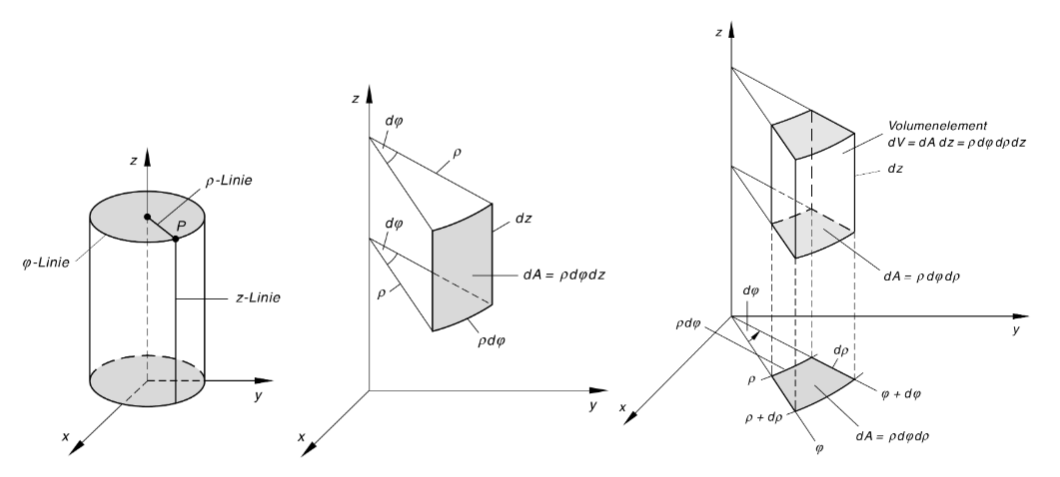
\includegraphics[width=\textwidth]{../pictures/Zylinderkoordinaten.png}

\subsection{Kugelkoordinaten}
\textbf{Flächenelement:} $dA=r^2 \cdot sin \vartheta \ d\vartheta d\varphi \qquad A_{ges} = \int\limits_{0}^{2\pi} \int\limits_{0}^{\pi} r^2\cdot sin\theta \ d\theta d\varphi$\\
\textbf{Volumselement:} $dV= dAdr =r^2 \cdot sin \vartheta \ dr d\vartheta d\varphi \qquad V_{ges} = \int\limits_{0}^{2\pi} \int\limits_{0}^{\pi} \int\limits_{0}^{r}r^2\cdot sin\theta \ dr d\theta d\varphi$

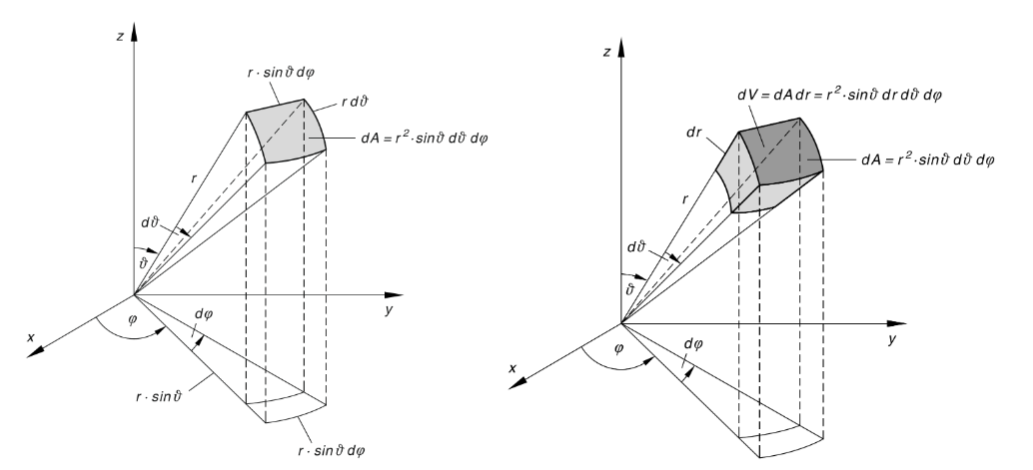
\includegraphics[width=.8\textwidth]{../pictures/Kugelkoordinaten.png}


\textbf{Schwerpunkt berechnen:} $R=\int \rho(\vec{r}) \cdot \vec{r}\ dV = \int\limits_{0}^{2\pi} \int\limits_{0}^{\pi} \int\limits_{0}^{r} \rho(\vec{r}) \cdot \vec{r}\ dr d\theta d\varphi$